\documentclass[12pt,a4paper]{report}
\usepackage[utf8]{inputenc}
\usepackage[english]{babel}
\usepackage{amsmath}
\usepackage{amsfonts}
\usepackage{amssymb}
\usepackage{graphicx}
\usepackage{float}
\usepackage{cite}
\usepackage[left=2cm,right=2cm,top=2cm,bottom=2cm]{geometry}
\author{Eva María Urbano González\\}
\title{Consultative Committee for Space Data Systems (CCSDS)}
\begin{document}
\maketitle
\section{CCSDS}
\subsection{Mission and objectives}
The Consultative Committee for Space Data Systems was founded in 1982 to develop communications and data systems standards for spaceflight. The goal of CCSDS is to enhance governamental and commercial interoperability and cross-suport, while reducing risks during the communication. It also focuses its attention on reducing the time and the project costs.  For these reasons, a research through the CCSDS standards should be done for our project. Moreover, CCSDS recommendations are routinely submitted to the International Organization for Standardization (ISO) for adoption as international standards. In 1990 the CCSDS entered into a cooperative arrangement with ISO under which the CCSDS-developet recommendations are advanced to ISO TC20/SC13 where they are progressed into ISO/CCSDS Standards. 
\subsection{Space Link Services Area}
The SLS (Space Link Services) works developing efficient space link communication systems. As we already know, a space link interconnects a spacecraft with its ground station and with other satellites. In this section is possible to find protocols like the AOS Space Data Link Protocol, which is a protocol to be used over space-to-ground, ground-to-space, or space-to-space communication links.\cite{CC2006}  
\bibliographystyle{plain} 
\subsection{AOS}
As it has been said in the previous paragraph, the AOS Space Data Link Protocol is a Data Link Layer Protocol that has been designed to meet the requirements of space missions. The AOS Space Data Link Protocol corresponds to the Data Link Protocol Sublayer, and provides functions of transverring various data usign a fixed-lenght protocol data unit called Transfer Frame. In the following illustration is possible to observe the relationship between this protocol and the reference model of OSI (Open Systems Interconnection).
\begin{figure}[H]
\centering
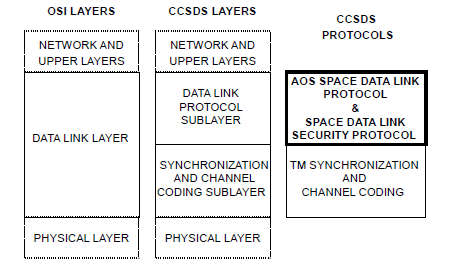
\includegraphics[scale=1]{AOS.PNG} 
\caption{Relationship between AOS and OSI protocol}
\end{figure}
Now the main features of this protocol will be exposed in order to know whether is adequated or not to our application.
\paragraph{Transfer Frames and Virtual Channels}
Fixed-lenght data units are used to transfer data trough the links. These protocol data units are known as Transfer Frames, and each of them contains a header which provides protocol control information and a fixed-lenght data field. Another important aspect of the AOS protocol is the concept of Virtual Channel (VC). A single Physical Channel is divided into several separate logical data channels, each of them known as Virtual Channels. VC allows one Physical Channel to be shared among multiple higher-layer data streams. Each Transfer Frame trasnferred over a Physical Channel belongs to one of its Virtual Channels.
\paragraph{Adressing}
There are headings in the Transfer Frames to know where are they going. This heading is composed by three identifier fields: transfer frame version number (TFVN), spacecraft identifier (SCID) and virtual channel identifier (VCID).The concatenation of a TFVN and a SCID is known as a Master Channel Identifier (MCID), and the concatenation of an MCID and a VCID is called a Global Virtual Channel Identifier (GVCID). All the same Transfer Frames with the same MCID on a Physical Channel constitute a Master Channel. A MC constist of several virtual channels. Let's see more clearly this relations: 
\begin{figure}[H]
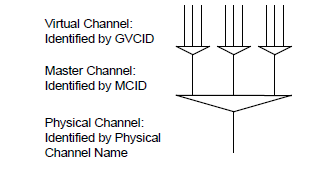
\includegraphics[scale=1]{relationschannels.PNG} 
\centering
\caption{Channels relationships}
\end{figure}
\paragraph{Features}
Now that we know the most important things about the data transmission of this protocol, the features defined by the standard are exposed:
\begin{itemize}
\item Unidirectional services: One end of a connection can send but not receive data through the space link, and the same in the opposite case.
\item Unconfirmed services: Sending user does not receive confirmation from the receiveng end that the data has arrived succesfully.
\item Incomplete services: The services do not guarantee completeness.
\item Sequence-preserving services: The sequence of service data units supplied by the sending user is preserved through the transfer over the space link.
\end{itemize} 
After knowing the features that this protocol can offer, we decide to decline it as it does not accomplish what has been fixed during the elaboration of communications logistics. However, this protocol can be useful in terms of headings for the transferred data and the idea of virtual channels. 
\bibliography{CC2006}
\end{document}